\begin{figure}[tbp] 
  \centering
  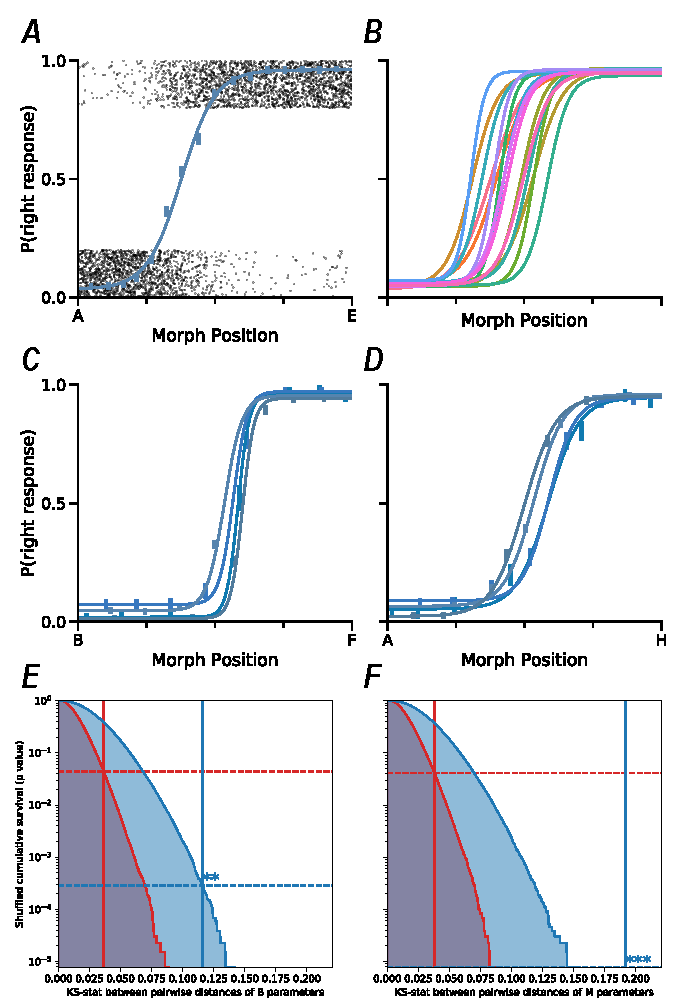
\includegraphics[width=114mm]{figures/fig02_conserved.pdf}
  \caption[Psychometric curves are conserved among different birds]
{(continued on following page.)
\index{conserved}}
  \label{fig:conserved}
\end{figure}

\begin{figure}[tp]
  \contcaption{
(A)	Construction of a single psychometric curve: The x-axis represents presentations of stimuli that vary between motif A on the left and motif E on the right. The middle tick mark is the location of a stimuli that lies exactly between motif A and motif E (according to the \DBN). Thus the 3 tick marks indicate the location of stimuli that is (left) 75\% A, 25\% E, (middle) 50\% A, 50\% E, and (right) 25\% A, 75\% E. The y-axis is the probability of a right response (that has been operantly conditioned to be associated with motif E). The black dots represent the binary decision of the birds (responses are jittered to demonstrate relative density). All the responses ordered by morph position are binned into 16 equally sized bins and the 95\% confidence intervals of the mean estimates are plotted as vertical blue lines. The maximum-likelihood 4 parameter logistic fit of the probability of the bird responding right as a function of morph position between motif A and motif E, which we will call the psychometric curve, is plotted in blue.
(B)	Psychometric curve variation: The set of all 16 behaviorally determined psychometric curves for a single bird. Color indicates each of the 16 different morph dimensions
(C-D)	Exemplar psychometric curves that are conserved between subjects: 2 of the 16 morph dimensions, (C) motif B to motif F and (D) motif A to motif H, are plotted for 4 different birds trained on the same categorization task. The full 16 dimensions are plotted in supplemental figure \ref{}
(E)	To measure how the B parameter (determines boundary sensitivity or slope at the boundary) of the psychometric curves is grouped we take the one-sided \KS metric between the distribution of pairwise distances between the B parameter of all psychometric curves, to the distribution of pairwise distances between the B parameter of psychometric curves from the same morph dimension (blue), and to the distribution of pairwise distances between the B parameter of psychometric curves from the same bird (red). The vertical blue line represents the \KS statistic between the distribution of pairwise distances between psychometric sensitivities that share the same morph dimension to that of all measured psychometric curves. The blue shaded cumulative survival curve is the distribution of expected \KS statistic values if we randomly split the psychometric curves into groups that share the same size as the morph dimension groups, or the null distribution as estimated by $2^{17}=131,072$ shuffles. Thus, the interception of the vertical blue line with the blue shaded cumulative survival curve provides an estimate of the likelihood that the psychometric sensitivities are as close to the psychometric sensitivities of other birds on the same morph dimension by chance, $p=3E-4$. We use an 8-way bonferroni correction to account for the 2 groupings and 4 parameters we test. * indicates $p<0.00625$, **, $p<0.00125$, and ***, $p<0.000125$. The vertical red line is the \KS statistic between the distribution of pairwise distances between psychometric sensitivities from the same bird to the distribution of pairwise distances between all psychometric sensitivities. Its corresponding shuffled null distribution is plotted as the red shaded region providing an estimate of $p=0.044$. Together, this indicates that psychometric sensitivities are closer than would be expected by chance when grouped by morph dimension, but not when grouped by bird.
(F)	The corresponding figure for the M parameter (boundary location). This shows that the likelihood that the psychometric boundaries are as close to the psychometric boundaries of other birds on the same morph dimension by chance (blue), $p<8E-6$ because never once in all the $2^{17}$ shuffles, was the KS statistic as great as the value measured. When distances between psychometric boundaries within a single bird are considered (red), $p=0.041$. This indicates that psychometric boundaries are also closer than would be expected by chance when grouped by morph dimension, but not when grouped by bird. Parameters A and K, the maximum accuracy achieved near each endpoint, are plotted in supplemental figure \ref{} and show the opposite trend.
}
\end{figure}